%
% main.tex -- Paper zum Thema <gamma>
%
% (c) 2020 Autor, OST Ostschweizer Fachhochschule
%
% !TEX root = ../../buch.tex
% !TEX encoding = UTF-8
%
\chapter{Die Gamma-Funktion\label{chapter:gamma}}
\kopflinks{Die Gamma-Funktion}
\begin{refsection}
\chapterauthor{Lukas Buchli und Roman Weber}

\index{Lukas Buchli}%
\index{Buchli, Lukas}%
\index{Roman Weber}%
\index{Weber, Roman}%

% Ein paar Hinweise für die korrekte Formatierung des Textes
% \begin{itemize}
% \item
% Absätze werden gebildet, indem man eine Leerzeile einfügt.
% Die Verwendung von \verb+\\+ ist nur in Tabellen und Arrays gestattet.
% \item
% Die explizite Platzierung von Bildern ist nicht erlaubt, entsprechende
% Optionen werden gelöscht. 
% Verwenden Sie Labels und Verweise, um auf Bilder hinzuweisen.
% \item
% Beginnen Sie jeden Satz auf einer neuen Zeile. 
% Damit ermöglichen Sie dem Versionsverwaltungssysteme, Änderungen
% in verschiedenen Sätzen von verschiedenen Autoren ohne Konflikt 
% anzuwenden.
% \item 
% Bilden Sie auch für Formeln kurze Zeilen, einerseits der besseren
% Übersicht wegen, aber auch um GIT die Arbeit zu erleichtern.
% \end{itemize}

\noindent
Die Gamma-Funktion, normalerweise geschrieben als $\Gamma$, ist eine Erweiterung des Definitionsbereichs der Fakultät.
\index{Fakultat@Fakultät}%
Die Fakultät ist nur für natürlichen Zahlen definiert.
Es stellt sich die Frage, warum eine solche Erweiterung überhaupt wünschenswert ist.
Wir wollen eine Motivation anhand der Berechnung von Kugelvolumen geben.
Es wird demonstriert, dass das Volumen einer $n$-dimensionalen Kugel anhand des Volumens einer tiefer-dimensionalen Kugel berechnet werden kann.
Durch diese rekursive Struktur folgt ganz natürlich die Verwendung der Gamma-Funktion,
da diese unter anderem durch ihre rekursive Eigenschaft ausgezeichnet ist.

Das Auftreten der Gamma-Funktion in der Berechnung von Kugelvolumen erklärt zudem die Notwendigkeit von auf den ersten Blick erstaunlichen Resultaten wie
\index{Gamma-Funktion}%
$\Gamma(\frac{1}{2}) = \sqrt{\pi}$.

\section{Rekursive Eigenschaft der Kugelvolumen\label{gamma:section:spheres}}
\kopfrechts{Kugelvolumen}

$\pi$ ist definiert als die Konstante, welche
\index{pi@$\pi$}%
\begin{equation}
\label{gamma-eq:circumference}
    2 \pi r = \text{Umfang eines Kreises mit dem Radius $r$}
\end{equation}
erfüllt.

Eine Kreisscheibe ist die von einem Kreisrand begrenzte, vollständig ausgefüllte Fläche eines Kreises.
\index{Kreisscheibe}%
Mit Hilfe von \eqref{gamma-eq:circumference} lässt sich die Fläche einer Kreisscheibe herleiten. 
Geht die Breite eines Rings gegen 0, verhält sich das 
Wachtstum des Flächeninhalts gleich wie das des Umfangs des Rings.
Das macht eine Herleitung der Kreisscheibenfläche per Integral möglich:
\begin{equation}
\label{gamma-eq:area}
    A(r) = \int_{0}^{r} 2 \pi r \,dr = \pi r^2
.
\end{equation}
Für eine grafische Darstellung dieser
Intuition siehe Abb. \ref{gamma-fig:ring-integration}.

Der Satz des Pythagoras gibt uns eine einfache Beschreibung aller
\index{Pythagoras}%
Punkte $(x, y)$, welche
\begin{equation}
\label{gamma-eq:pythagoras}
    x^2 + y^2 \leq r^2
\end{equation}
erfüllen und somit Teil des Kreises mit Radius $r$ sind.

Aufgrund der Ungleichung~\eqref{gamma-eq:pythagoras}
lässt sich eine weitere Definition der Kreisfläche herleiten, 
indem wir nach $y$ auflösen und danach für jedes $x$ den jeweils höchsten $y$-Wert integrieren:
\begin{gather}
\label{gamma-eq:pythagoras-y}
    y \leq \!\sqrt{r^2 - x^2} \\
\label{gamma-eq:area-pythagoras}
    A(r) = 2 \int_{-r}^{r} \!\sqrt{r^2-x^2} \,dx.
\end{gather}
Die Intuition dahinter wird in Abb.~\ref{gamma-fig:rect-integration} dargestellt.
Das Integral aus~\eqref{gamma-eq:area-pythagoras} ist nicht trivial zu lösen
und wird nicht weiter verfolgt.
Ein Vorteil ist, dass sich die durch den Satz des Pythagoras definierte Metrik
einfach auf weitere Dimensionen erweitern lässt, beispielsweise mit
\begin{equation}
\label{gamma-eq:pythagoras-3d}
    \begin{split}
    x^2 + y^2 + z^2 \leq r^2 \\
    z \leq \!\sqrt{r^2 - x^2 - y^2}
    \end{split}
\end{equation}
auf 3 Dimensionen.

Nun können wir das Volumen einer Kugel herleiten, indem wir Halbzylinder entsprechender
Grösse entlang $x$ integrieren (siehe Abb. \ref{gamma-fig:semicircle-integration}),
während iterativ in jedem Halbkreis entlang der $y$-Achse integriert wird. Das Volumen kann also mit
\begin{equation}
\label{gamma-eq:sphere-volume}
    V(r) = 2 \int_{-r}^{r} \int_{-\!\sqrt{r^2-x^2}}^{\!\sqrt{r^2-x^2}} \sqrt{r^2-x^2-y^2} \,dy \,dx
\end{equation}
berechnet werden. Eine formelle Begründung für diese iterative angehensweise ist der Satz von Fubini \cite{fubini1907integrali}.
\index{Satz!von Fubini}%
\index{Fubini, Satz von}%
Die Grenzen des inneren Integrals kommen zustande, weil für ein bestimmtes $x$ die möglichen $y$-Werte gemäss Ungleichung~\eqref{gamma-eq:pythagoras-y} eingeschränkt sind.
Für ein bestimmtes $x$ und $y$ wird dann über den maximalen Wert für $z$ gemäss Ungleichung~\eqref{gamma-eq:pythagoras-3d} integriert.

\input{papers/gamma/spheres_drawings.tex}

Da wir aber bereits die Fläche eines Kreises berechnen können, können wir $A(r)$
zur Berechnung des Kugelvolumens anstatt der Pythagoras-Methode verwenden, indem wir in
\begin{equation}
\label{gamma-eq:composed-sphere-volume}
    V(r) = 2 \int_{-r}^{r} A\left(\!\sqrt{r^2-x^2}\right) \,dx
\end{equation}
das innere Integral von~\eqref{gamma-eq:sphere-volume} durch die entsprechende Flächenberechnung ersetzen.
Das ist interessant, weil wir die Berechnung für zwei Dimensionen verwendet haben,
um das Volumen in drei Dimensionen zu berechnen.

Auf die gleiche Weise lässt sich das Volumen auf beliebige Dimensionen $> 2$ erweitern,
und zwar mit
\begin{equation}
\label{gamma-eq:n-sphere-volume-recursive}
    V_{n+1}(r) = \int_{-r}^{r} V_n\left(\!\sqrt{r^2-x^2}\right) \,dx
.
\end{equation}

\noindent
Betrachtet man $A(r) = V_2(r) = 2 \pi r$, so scheint es intuitiv,
dass $V_n$ jeweils mit $C_n r^n$ dargestellt werden kann, wobei $C_n$ eine der Dimension zugehörige Konstante ist.
Wir können induktiv beweisen, dass $V_{n+1}$ dieser Form entspricht, sofern
$V_n$ dieser Form entspricht.
Nehme an, dass $V_n(r) = C_n r^n$. Dann gilt:

\begin{align*}
%\label{gamma-eq:const-structure-induction}
         V_{n+1}(r) &= \int_{-r}^{r} C_n \left(\!\sqrt{r^2-x^2}\right)^n \,dx  \\ 
        &= \int_{-r}^{r} C_n \left(r^2-x^2\right)^{n/2} \,dx \\
        &= \int_{-1}^{1} C_n \left(r^2 - (ru)^2\right)^{n/2} r \,du \\
        &= \int_{-1}^{1} C_n \left(r^2 (1 - u^2)\right)^{n/2} r \,du \\
        &= \int_{-1}^{1} C_n r^{n+1} (1- u^2)^{n/2} \,du \\
        &= r^{n+1} \underbrace{C_n \int_{-1}^{1} (1- u^2)^{n/2} \,du}_{C_{n+1}}.
\end{align*}

\noindent
Wir sehen, dass $C_n$ ein Faktor von $C_{n+1}$ ist. Die mit dem Volumen assoziierte Konstante 
scheint also eine rekursive Struktur ähnlich der einer Fakultät aufzuweisen. Eine Untersuchung des Terms $I_n = \int_{-1}^1 (1- u^2)^{n/2} \,du$ ergibt weiter die rekursive Struktur $I_n = \frac{n}{n+1} I_{n-2}$. Dies kann durch die Rechnung
\begin{align*}
%\label{gamma-eq:n-sphere-constant}
        I_n &= \int_{-1}^1 (1- u^2)^{n/2} \,du
\\
        &= \left[ u (1-u^2)^{n/2} \right]_{-1}^{1} - \int_{-1}^1 u \cdot (-nu(1-u^2)^{n/2 - 1}) \,du
\\
        &= (0 - 0) - \int_{-1}^1 -nu^2(1-u^2)^{n/2 - 1} \,du
\\
        &= n \int_{-1}^1 u^2 (1 - u^2)^{n/2 - 1} \,du
\\
        &= n \int_{-1}^1 (1 - (1 - u^2)) (1-u^2)^{n/2 - 1} \,du
\\
        &= n \int_{-1}^1 (1 - u^2)^{n/2 - 1} \,du - n \int_{-1}^1 (1-u^2)^{n/2} \,du
\\
        &= n I_{n-2} - n I_n \\
        (n+1) I_n &= n I_{n-2} \\
        I_n &= \frac{n}{n+1} I_{n-2}
\end{align*}
gezeigt werden.

Mit diesem Wissen lässt sich der konstante Faktor des Volumens einer $n$-dimensionalen Kugel herleiten als
$C_n = C_{n-1} I_{n-1} = C_{n-2} I_{n-1} I_{n-2} = C_{n-2} \frac{2}{n} I_1 I_0$.
Der letzte Schritt ist durch
\begin{align}
    I_{n-1} I_{n-2}
&=
\biggl(\frac{n-1}{n} \cdot \frac{n-3}{n-2} \cdot \ldots \cdot \frac{3}{4}
\cdot I_1\biggr)
\cdot
\biggl(\frac{n-2}{n-1} \cdot \frac{n-4}{n-2} \cdot \ldots \cdot \frac{2}{3} \cdot I_0\biggr)
\notag\\
    &= \frac{n-1}{n} \cdot \frac{n}{n-1} \cdot \ldots \cdot \frac{3}{4} \cdot  \frac{2}{3} \cdot I_1 I_0
\label{gamma-eq:n-sphere-constant-2}
\\
    &= \frac{2}{n} \cdot I_1 I_0
\notag
\end{align}
begründet, funktioniert aber nur mit geraden $n$.

Von~\eqref{gamma-eq:area} wissen wir, dass $C_2 = \pi$.
Eine einfache Rechnung ergibt, dass $I_0 = 2$ und $I_1 = \frac{\pi}{2}$, d.h. $C_n = C_{n-2} \frac{2 \pi}{n}$.
Jetzt können wir für gerade Dimensionen die rekursive Definition `abrollen' in einen einzigen
Term:
\begin{equation}
\label{gamma-eq:nonrecursive-constant}
\begin{split}
        C_n &= \pi \cdot \frac{2 \pi}{4} \cdot \frac{2 \pi}{6} \cdot \ldots \cdot \frac{2 \pi}{n} \\
            &= \frac{2 \pi}{2} \cdot \frac{2 \pi}{4} \cdot \frac{2 \pi}{6} \cdot \ldots \cdot \frac{2 \pi}{n} \\
            &= \frac{(2 \pi)^{n/2}}{2^{n/2}} \frac{1}{\left(\frac{n}{2}\right)!} \\
            &= \frac{\pi^{n/2}}{\left(\frac{n}{2}\right)!}.
\end{split}
\end{equation}
Wir können jetzt also mit
\begin{equation}
\label{gamma-eq:n-sphere-volume-even}
    V_n(r) = \frac{\pi^{n/2}}{(\frac{n}{2})!}  r^n
\end{equation}
ein Kugelvolumen bei geraden Dimensionen einfach berechnen.

Schön wäre es, das Volumen nicht nur für gerade-dimensionale Kugeln berechnen können.
Dazu müssten wir allerdings die Fakultät auf halbe Zahlen anwenden können, was einer der Gründe ist, die Fakultät zu erweitern.

%
% einleitung.tex -- Beispiel-File für die Einleitung
%
% (c) 2020 Prof Dr Andreas Müller, Hochschule Rapperswil
%
% !TEX root = ../../buch.tex
% !TEX encoding = UTF-8
%
\section{Die $\Gamma$-Funktion als Erweiterung der Fakultät\label{gamma:section:teil0}}
\kopfrechts{Fakultät erweitern}

Die Erweiterung der Fakultät beschäftigt grosse Namen der Mathematik schon lange.
Eine erste Definition der Fakultät für nicht natürliche Zahlen wird bereits 1720 von Daniel Bernoulli und Christian Goldbach gegeben.
\index{Goldbach, Christian}%
\index{Bernoulli, Daniel}%
Auch Leonhard Euler und James Stirling steuern im Laufe der Jahrhunderte ihre eigene Definition bei. 
\index{Euler, Leonhard}%
\index{Stirling, James}%

\subsection{Bohr-Mollerup-Theorem}\label{gamma:section:BMT}

Um eine Funktion zu finden, welche die Fakultät erweitert, wird das Bohr-Mollerup-Theorem \cite{mollerup1922laerebog} verwendet. Es werden folgende Eigenschaften definiert:
\index{Bohr, Harald}%
\index{Mollerup, Johannes}%
\index{Satz!von Bohr-Mollerup}%

\begin{enumerate}
\item\label{gamma-eq:bm-1}$f(1) = 1$,
\item\label{gamma-eq:bm-2}$f(x+1) = x \cdot f(x), x > 0$,
\item\label{gamma-eq:bm-3}$f(x) \text{ ist logarithmisch konvex}$.
\end{enumerate}

\noindent
Eine Funktion, welche die Eigenschaften~\ref{gamma-eq:bm-1},~\ref{gamma-eq:bm-2} und~\ref{gamma-eq:bm-3} erfüllt,
kann als Erweiterung der Fakultät für nicht natürliche Zahlen betrachtet werden.

Die Eigenschaft~\ref{gamma-eq:bm-1} ist selbsterklärend.
Die Eigenschaft~\ref{gamma-eq:bm-2} verlangt, dass die Funktion rekursiv definiert werden kann.
Die Fakultät erfüllt das, da $5! = 5 \cdot 4!$ ist.
Die Eigenschaft~\ref{gamma-eq:bm-3} verlangt logarithmische Konvexität, was informell als ``wächst schnell'' verstanden werden kann.
Die formelle Definition folgt im nächsten Abschnitt.

\subsubsection{Logarithmische Konvexität}

Eine Kurve ist konvex, wenn diese wie $f(x) = x^2+1$ nach oben geöffnet ist.
Von \emph{logarithmischer Konvexität} spricht man wenn, nach der Anwendung des Logarithmus, die resultierende Funktion auch konvex ist. 
\index{logarithmisch konvex}%
Die Funktion $f(x) = x^2+1$ ist zum Beispiel nicht logarithmisch konvex, denn die zweite Ableitung des Logarithmus ist stellenweise negativ, wie die Abb. \ref{gamma-fig:nonLogConvex} aufzeigt.

\begin{figure}
  \centering
  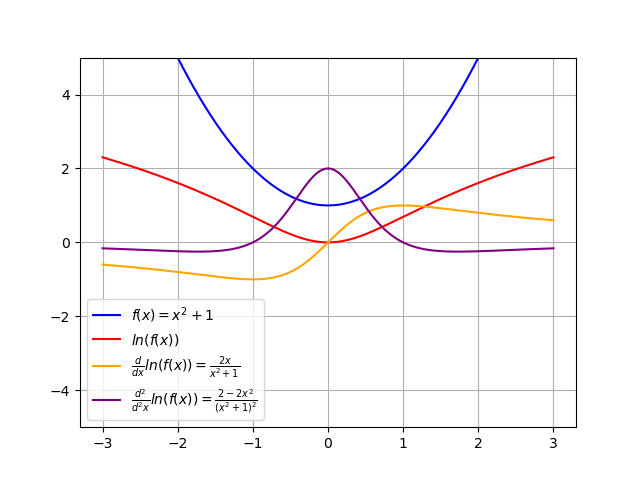
\includegraphics[width=0.8\textwidth]{papers/gamma/img/log_nonconvex.png}
  \caption{Visualisierung der nicht erfüllten logarithmischen Konvexität von $f(x) = x^2+1$.}
\label{gamma-fig:nonLogConvex}
\end{figure}

Ein Beispiel einer logarithmisch konvexen Funktion ist
\begin{equation}
  \label{gamma-eq:logConvex}
  g(x) = e^{x^2} \quad \Rightarrow \quad \log(g(x)) = \log\left(e^{x^2}\right) = x^2,
\end{equation}
deren logarithmische Konvexität auch in Abb. \ref{gamma-fig:logConvex} dargestellt wird.

\begin{figure}
  \centering
  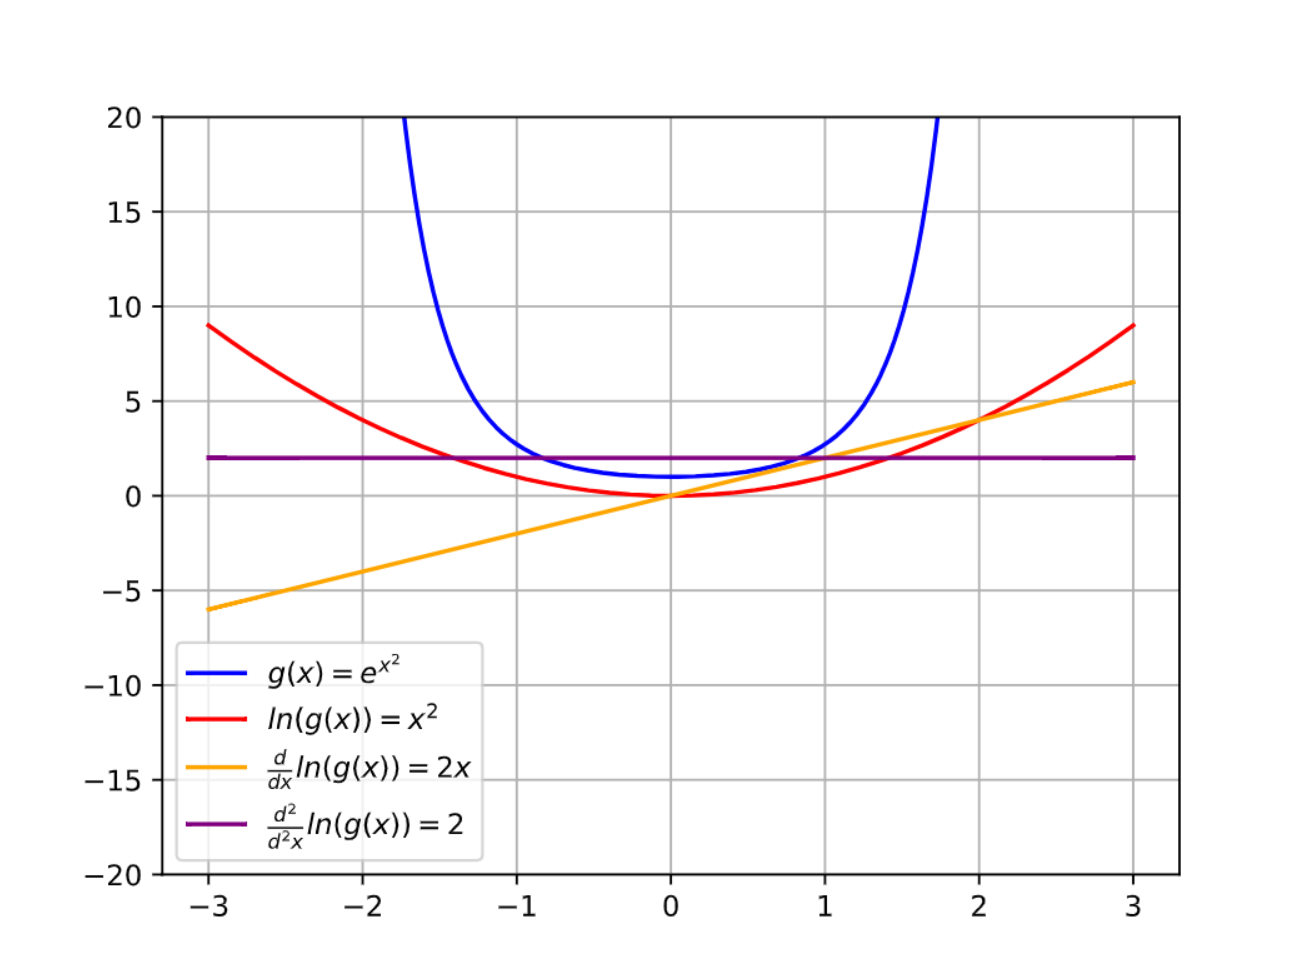
\includegraphics[width=0.8\textwidth]{papers/gamma/img/log_convex_3.png}
  \caption{Visualisierung der logarithmischen Konvexität von $g(x) = e^{x^2}$.}
\label{gamma-fig:logConvex}
\end{figure}

\subsubsection{Suche nach einer passenden Funktion}

Eine Funktion, welche Eigenschaften \ref{gamma-eq:bm-1} und \ref{gamma-eq:bm-2} erfüllt, lässt sich verhältnismässig leicht finden.
Als Beispiel, nimmt man die Funktion
\begin{equation}
\label{gamma-eq:sinusFunction}
    f : \interval[open left, soft open fences]{0}{1} \to \mathbb{R} \quad x \mapsto 2\sin(2 \pi x)+1,
\end{equation}
wird Eigenschaft~\ref{gamma-eq:bm-1} durch die Verschiebung nach rechts bereits erfüllt. Sie kann dann gemäss Eigenschaft~\ref{gamma-eq:bm-2} rekursiv auf
\begin{equation}
\label{gamma-eq:rec-sinus-function}
    \tilde{f} : \mathbb{R} \to \mathbb{R} \quad x \mapsto \begin{cases}
        x^{-1} \cdot f(x+1) & x \leq 0 \\
        2\sin(2 \pi x)+1   & 0 < x \leq 1 \\
        x \cdot f(x-1)     & x > 1
\end{cases}
\end{equation}
erweitert werden und erfüllt somit diese auch.

Wie die Grafik~\ref{gamma-fig:almostGammaFunction} zeigt, nimmt~\eqref{gamma-eq:rec-sinus-function} die bekannten Fakultätswerte an.
Die Ausschläge nach unten und oben zeigen grafisch, dass die logarithmische Konvexität (Eigenschaft~\ref{gamma-eq:bm-3}) für diese Funktion nicht gegeben sein kann.

\begin{figure}
  \centering
  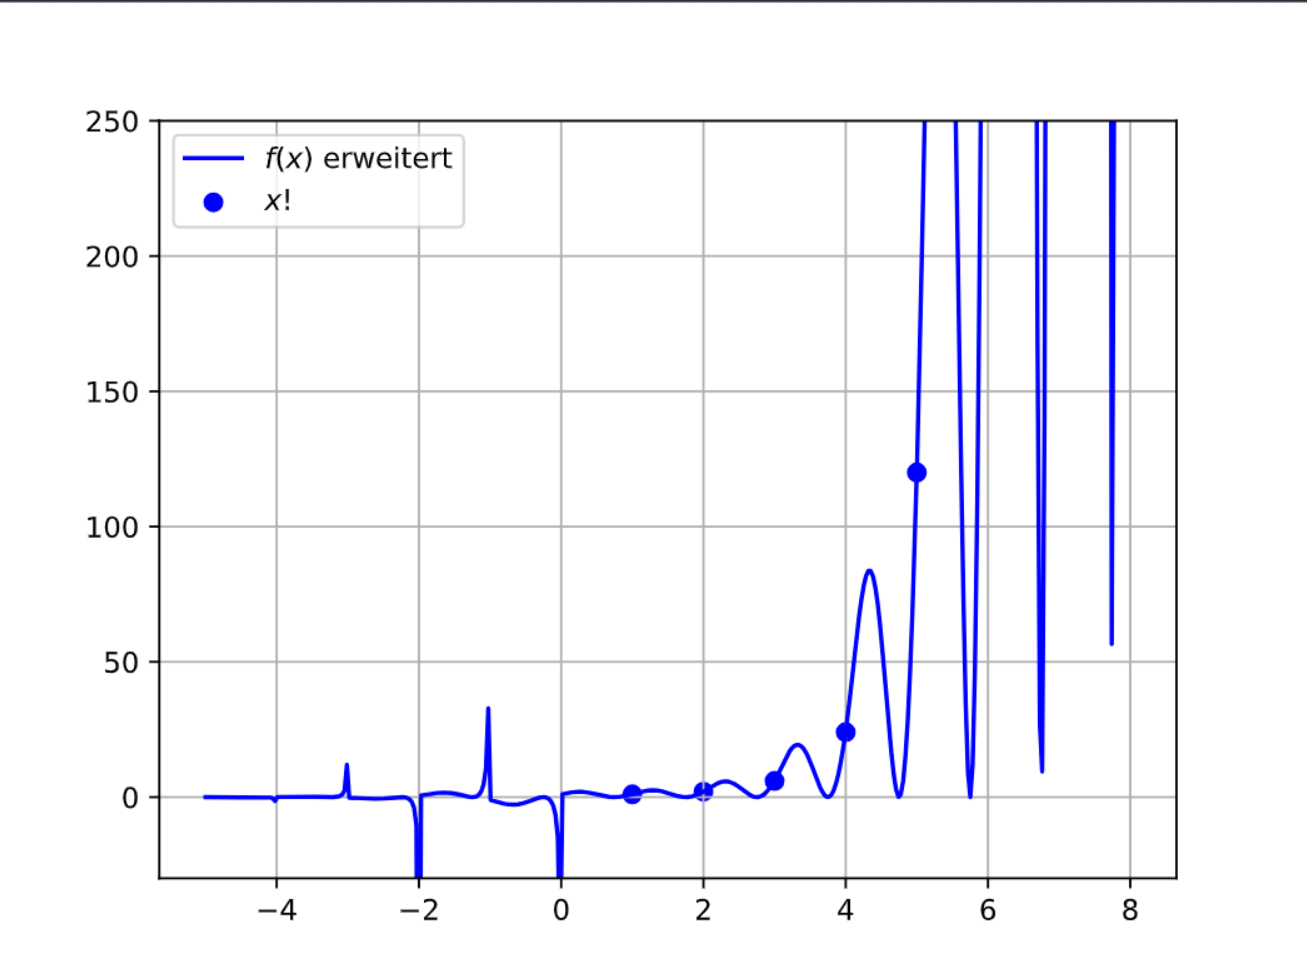
\includegraphics[width=0.8\textwidth]{papers/gamma/img/sin_extended.png}
  \caption{Funktion $f(x)$, welche zwei (\ref{gamma-eq:bm-1} und~\ref{gamma-eq:bm-2}) von drei Eigenschaften des Bohr-Mollerup-Theorems erfüllt.}
\label{gamma-fig:almostGammaFunction}
\end{figure}

Gesucht wird eine Funktion, welche alle Eigenschaften, welche als Teil des Bohr-Mollerup-Theorems definiert wurden, erfüllt.
Die Herleitung der $\Gamma$-Funktion ist nicht trivial und wird deshalb weggelassen (Beispiele in \ref{gamma:section:formulas}).
\index{Gamma@$\Gamma$}%
Interessant ist die Hauptaussage des Bohr-Mollerup-Theorems: die $\Gamma$-Funktion erfüllt als einzige Funktion alle Eigenschaften und ist somit die eindeutige Erweiterung der Fakultät \cite{mollerup1922laerebog}.

\section{Formeln zur $\Gamma$-Funktion\label{gamma:section:formulas}}
\kopfrechts{Formeln zur $\Gamma$-Funktion}

Für die $\Gamma$-Funktion existieren verschiedene Darstellungen und Näherungsverfahren.
Im Folgenden werden ausgewählte Formeln sowie ihre jeweiligen Anwendungsgebiete vorgestellt, wobei auf ausführliche mathematische Herleitungen verzichtet wird.
Abschliessend wird die Bedeutung der $\Gamma$-Funktion für die Berechnung des Kugelnvolumens aufgezeigt.

\subsection{Produktformel von Euler}

Auf der Suche nach der $\Gamma$-Funktion im 18. Jahrhundert hat Leonhard Euler unendliche Produkte verwendet.
Mit Hilfe des Bohr-Mollerup-Theorems (Abschnitt~\ref{gamma:section:BMT}) kann nachgewiesen werden, dass es sich bei
\index{Produktformel, Gamma-funktion}%
\index{Gamma-Funktion!Produktformel}%
\index{Gamma-Funktion!Euler-Formel}%
\begin{equation}
\label{gamma-eq:product-formula-euler}
    \Gamma_{\text{Euler}}(z) = \lim_{n \to \infty} \frac{n!\,n^z}{z(z+1)\cdots(z+n)}
\end{equation}
um die $\Gamma$-Funktion handelt.

Die erste Eigenschaft des Bohr-Mollerup-Theorem lässt sich durch Einsetzen von $z=1$ überprüfen:
\begin{equation}
\label{gamma-eq:euler-first-property}
    \begin{split}
    \Gamma_{\text{Euler}}(1)
        &= \lim_{n \to \infty} \frac{n!\,n}{1 \cdot 2 \cdots (n+1)} \\
        &= \lim_{n \to \infty} \frac{n!\,n}{(n+1)!} \\
        &= \lim_{n \to \infty} \frac{n}{n+1} \\
        &= 1.
    \end{split}
\end{equation}
Für die zweite Eigenschaft wird $z+1$ anstelle von $z$ eingesetzt. Durch Umformen erhält man
\begin{equation}
\label{gamma-eq:euler-recursive-property}
    \begin{split}
    \Gamma_{\text{Euler}}(z+1)
        &= \lim_{n \to \infty}
            \frac{n!\,n^{z+1}}{(z+1)(z+2)\cdots(z+n+1)} \\
        &= \lim_{n \to \infty}
            \biggl(
            \frac{n}{z+n+1}
            \cdot
            \frac{n!\,n^z}{(z+1)(z+2)\cdots(z+n)}
            \biggr) \\
        &= \lim_{n \to \infty}
            \frac{n}{z+n+1}
            \cdot z
            \frac{n!n^{z}}{z(z+1)(z+2)\cdots(z+n)} \\
        &= \lim_{n \to \infty} \frac{n}{z+n+1}
            \cdot z\Gamma_{\text{Euler}}(z) \\
        &= z\Gamma_{\text{Euler}}(z).
    \end{split}
\end{equation}
Damit erfüllt die Produktformel die Eigenschaften~\ref{gamma-eq:bm-1} und~\ref{gamma-eq:bm-2}.
Jetzt muss man noch zeigen, dass $\Gamma_{\text{Euler}}$ gemäss Eigenschaft~\ref{gamma-eq:bm-3} logarithmisch konvex ist.
Die Log-Konvexität der Produktdarstellung wird im Standardbeweis des Satzes von Bohr-Mollerup bewiesen \cite[Abschnitt 4.1.4]{buch:MatSeSspezielleFunktionen}.
Nach dem Satz von Bohr-Mollerup gilt $\Gamma_{\text{Euler}}(z) = \Gamma(z)$.

\subsection{Integraldarstellung}

Die Integraldarstellung
\index{Integraldarstellung, Gamma-Funktion}%
\index{Gamma-Funktion!Integraldarstellung}%
\begin{equation}
\label{gamma-eq:integral}
    \Gamma_{\text{Integral}}(z) = \int_0^\infty t^{z-1} e^{-t}\,dt,
    \qquad \operatorname{Re}(z)>0
\end{equation}
eignet sich besonders gut zur Untersuchung von Ableitungen. 
Auch $\Gamma_{\text{Intergal}}$ kann mit dem Eigenschaften vom Bohr-Mollerup-Theorem (\ref{gamma:section:BMT}) überprüft werden. 

Die erste Eigenschaft des Bohr-Mollerup-Theorems lässt sich durch Einsetzen von $z=1$ überprüfen:
\begin{equation}
\label{gamma-eq:integral-first-property}
    \begin{split}
    \Gamma_{\text{Integral}}(1)
        &= \int_0^\infty t^{1-1}e^{-t}\,dt \\
        &= \int_0^\infty e^{-t}\,dt \\
        &= \left[-e^{-t}\right]_0^\infty \\
        &= 1.
    \end{split}
\end{equation}
Für die zweite Eigenschaft wird $z+1$ anstelle von $z$ eingesetzt. Durch partielle Integration erhält man für $z>0$
\begin{equation}
\label{gamma-eq:integral-recursive-property}
    \begin{split}
    \Gamma_{\text{Integral}}(z+1)
        &= \int_0^\infty t^z e^{-t}\,dt \\
        &= \left[-t^z e^{-t}\right]_0^\infty
            + z\int_0^\infty t^{z-1}e^{-t}\,dt \\
        &= z\Gamma_{\text{Integral}}(z).
    \end{split}
\end{equation}
Damit erfüllt die Integraldarstellung die Eigenschaften~\ref{gamma-eq:bm-1} und~\ref{gamma-eq:bm-2}.

Mit der Ableitungsformel 
\begin{equation}
    \Gamma_{\text{Integral}}'(z)=\int_0^\infty t^{z-1}e^{-t}\log(t)\,dt.
\end{equation}
kann man auch die logarithmische Konvexität (\ref{gamma-eq:bm-3}) von $\Gamma_{\text{Integral}}(z)$ beweisen, wie in \cite[Abschnitt 4.1.5]{buch:MatSeSspezielleFunktionen} gezeigt.
Aus dem Satz von Bohr-Mollerup folgt dann, dass auch $\Gamma_{\text{Integral}}(z)=\Gamma(z)$.

\subsection{Lanczos-Approximation}

Die Lanczos-Approximation
\index{Gamma-Funktion!Lanczos-Approximation}%
\index{Lanczos-Approximation}%
\begin{equation}
\label{gamma-eq:lanczos}
    \Gamma_{\text{Lanczos}}(z) \approx \sqrt{2\pi}
    \biggl(z + g - \frac{1}{2}\biggr)^{z - \frac{1}{2}}
    e^{-(z + g - \frac{1}{2})}
    \biggl(c_0 + \sum_{k=1}^{N} \frac{c_k}{z + k - 1}\biggr)
\end{equation}
wurde 1964 von Cornelius Lanczos vorgestellt und wird heute häufig in numerischen Bibliotheken eingesetzt.
\index{Lanczos, Cornelius}%
Der Parameter $g$ und die Koeffizienten $c_k$ werden dabei im Voraus festgelegt und müssen nicht bei jeder Auswertung neu berechnet werden.
Da nur eine endliche Summe mit $N$ Gliedern ausgewertet wird, ermöglicht das Verfahren eine genaue und zugleich effiziente Berechnung der $\Gamma$-Funktion. 
Auch hier gilt $\Gamma_{\text{Lanczos}}(z) = \Gamma(z)$. 
Eine ausführliche Herleitung der Approximation sowie eine Analyse ihrer Genauigkeit finden sich in \cite{LanczosGammaApproximation}.

\section{Die $\Gamma$-Funktion im Kugelvolumen\label{gamma:section:teil0}}
\kopfrechts{$\Gamma$ in Kugelvolumen}
Da wir jetzt die $\Gamma$-Funktion kennen, können wir die Formel~\eqref{gamma-eq:n-sphere-volume-even} 
zur Berechnung des Kugelvolumens erweitern und alle Kugelvolumina mit
\begin{equation}
\label{gamma-eq:n-sphere-volume}
    V_n(r) = \frac{\pi^{n/2}}{\Gamma(\frac{n}{2}+1)}  r^n
\end{equation}
berechnen. 
Somit ist es nun auch möglich Kugelvolumina ungerader Dimensionen zu bestimmen.
Wir erfahren zum Beispiel, dass das Volumen einer $1$-dimensionalen Einheitskugel $V_1(1) = 2$ sein muss. 
Intuitiv ist das sinnvoll, wie Abb.~\ref{gamma-fig:1-dim-sphere} zeigt.

\begin{figure}
    \centering
    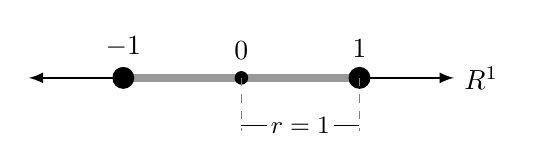
\begin{tikzpicture}[scale=1.5]
        \draw[latex-latex, thick, black] (-1.8, 0) -- (1.8, 0) node[right, black] {$\mathbb{R}^1$};
        \draw[line width=1mm, gray!80, cap=round] (-1, 0) -- (1, 0);
        \filldraw[black] (0,0) circle (1.5pt) node[above=3pt] {$0$};
        \filldraw[black] (-1,0) circle (2.5pt) node[above=4pt] {$-1$};
        \filldraw[black] (1,0) circle (2.5pt) node[above=4pt] {$1$};
        \draw[dimen/.style={<->, >=Latex, blue, thin}]
            (0, -0.4) -- node[fill=white, inner sep=1.5pt, font=\small] {$r = 1$} (1, -0.4);
        \draw[gray, dashed] (0, 0) -- (0, -0.45);
        \draw[gray, dashed] (1, 0) -- (1, -0.45);
    \end{tikzpicture}
    \caption{Die $1$-dimensionale Einheitskugel.}
    \label{gamma-fig:1-dim-sphere}
\end{figure}

Dieses Resultat hat die interessante Konsequenz, dass $\Gamma(\frac{3}{2}) = \frac{1}{2} \sqrt{\pi}$, weil sie $\sqrt{\pi}$ im Zähler ausgleichen muss.


\printbibliography[heading=subbibliography]
\end{refsection}
